\documentclass{article}
\usepackage{tikz}
\usetikzlibrary{automata,positioning,arrows}

% \tikzset{every edge/.append style={
%   auto,
% }}


\begin{document}

%
\section*{Automaton}

Input nfa from file {\tt example1.tikz}
\begin{center}
%% Machine generated by https://finsm.io
%% 2025-3-21-5:56:39
%% include in preamble:
%% (a#{a,b})#
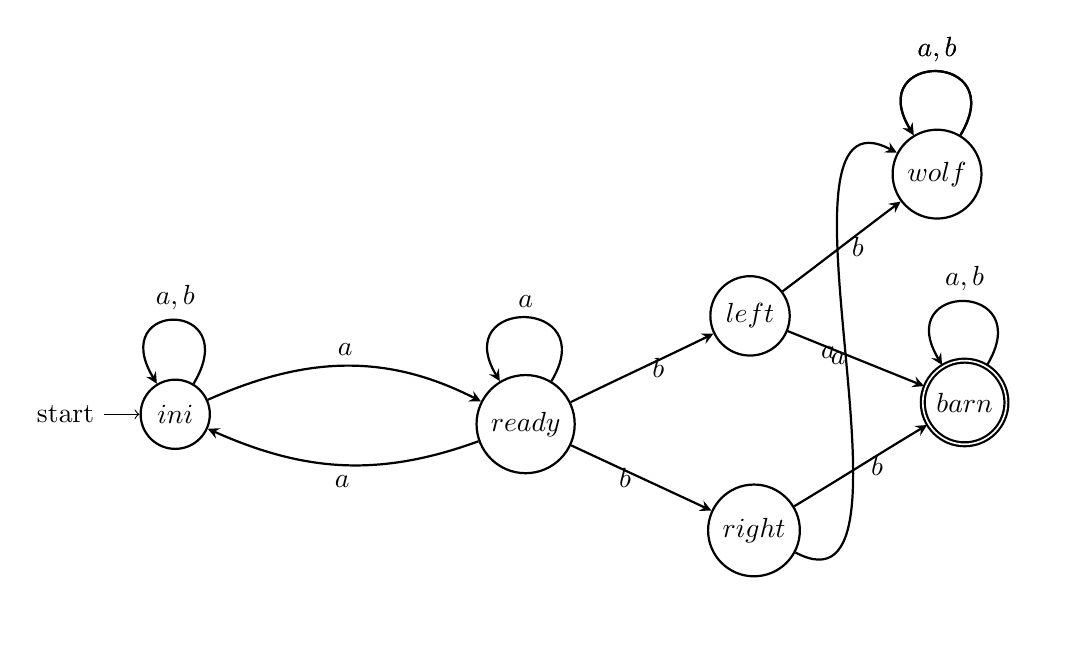
\begin{tikzpicture}[]
    \node[initial,thick,state] at (-3.175,4.95) (1fa0116c) {$ini$};
    \node[thick,state] at (1.275,4.825) (4c126865) {$ready$};
    \node[thick,accepting,state] at (6.85,5.1) (b8befb7d) {$barn$};
    \node[thick,state] at (4.125,6.2) (316b0ce4) {$left$};
    \node[thick,state] at (4.175,3.475) (6e65ff45) {$right$};
    \node[thick,state] at (6.5,8) (8a7c360d) {$wolf$};
    \path[->, thick, >=stealth]
    (1fa0116c) edge [loop,min distance = 1.25cm,above,in = 121, out = 59] node {$a,b$} (1fa0116c)
    (1fa0116c) edge [above,in = 153, out = 24] node {$a$} (4c126865)
    (4c126865) edge [loop,min distance = 1.25cm,above,in = 121, out = 59] node {$a$} (4c126865)
    (4c126865) edge [below,in = -24, out = -160] node {$a$} (1fa0116c)
    (4c126865) edge [right,in = -154, out = 26] node {$b$} (316b0ce4)
    (4c126865) edge [left,in = 155, out = -25] node {$b$} (6e65ff45)
    (b8befb7d) edge [loop,min distance = 1.25cm,above,in = 121, out = 59] node {$a,b$} (b8befb7d)
    (316b0ce4) edge [left,in = 158, out = -22] node {$a$} (b8befb7d)
    (316b0ce4) edge [right,in = -143, out = 37] node {$b$} (8a7c360d)
    (6e65ff45) edge [right,in = -149, out = 31] node {$b$} (b8befb7d)
    (6e65ff45) edge [left,in = 152, out = -28] node {$a$} (8a7c360d)
    (8a7c360d) edge [loop,min distance = 1.25cm,above,in = 121, out = 59] node {$a,b$} (8a7c360d)
    (8a7c360d) edge [loop,min distance = 1.25cm,above,in = 121, out = 59] node {$a,b$} (8a7c360d)
    ;
\end{tikzpicture}
 
\end{center}

Complete automaton:
\begin{verbatim}
States: { 0 , 1 , 2 , 3 , sink }
Initial: { 0 }
Accepting: { 3 }
Transitions:
        0 --a--> 1
        0 --a--> 2
        1 --a--> 3
        2 --b--> 3
        2 --a--> sink
        3 --a--> sink
        sink --a--> sink
        0 --b--> sink
        1 --b--> sink
        3 --b--> sink
        sink --b--> sink
\end{verbatim}

\newpage

\section*{Strategy}

The answer to the population control problem is:
\begin{verbatim}
					negative.
\end{verbatim}


\noindent Maximal winning random walk:
\begin{verbatim}
States:
		{ 0 , 1 , 2 , 3 , sink }

Play action 'a' in the downward-closure of
		( 1 , _ , _ , _ , _ )
		( _ , \omega , _ , _ , _ )


Play action 'b' in the downward-closure of
		( _ , _ , \omega , _ , _ )
\end{verbatim}

\end{document}
